\documentclass{ltjsbook}
\usepackage{docmute} 
\usepackage{../../myStyle} 

\begin{document}
\chapter{検定}
\label{ch13_NHST}
前回は標本から母平均を区間推定する方法について説明しました。今回は，これを使って「差があるかないか」という\textbf{判断}をする方法について考えます。

母平均を区間推定することで，「このあたりにある，と予測したらXX\%の確率で当たる」という範囲を定めることができました。この推定を実験群・統制群それぞれについて行うとすると，実験群の平均値はこの範囲，統制群の平均値はこの範囲にあると予測する，という言い方をすることになります。
その範囲が重複していなければ，実験群と統制群の平均値は異なると言い切れるでしょうが，信頼区間が重複することは当然起こり得ます。そのときどうやって「差がある」「差がない」という判断をするのか，ということが問題になるのです。
この判断は\keyterm{検定}{けんてい}{test}と呼ばれます。とくにその形式から，\keyterm{帰無仮説検定}{きむかせつけんてい}{Null Hypothesis Significance Test}，略して\textbf{NHST}と呼ばれます。

\label{ModelComparison1}
どこに注意が必要なのでしょうか？ いろいろな問題があるのですが，ここでは説明しながら代表的なものを1つ挙げてみましょう。検定は\underline{モデル比較}の考え方の一種です。統計的なモデル，というのは本講義の中では一貫して述べてきたように，データに対する理想形+誤差の考え方で，回帰分析に代表される線形的なモデルが代表的なものです。モデル比較とは，複数のモデルを用意した時にどちらのモデルがより良いか，という優劣を決めることです。統計的検定は，とくに\keyterm{帰無仮説検定}{きむかせつけんてい}{Null Hypothesis Significance Test}と呼ばれ，帰無仮説($H_0$と表記)と対立仮説($H_1$と表記)という2つのモデルを戦わせ，どちらが良いかを決定することにあります。

つまり，検定は「推定」に「判断」が加わったものです。判断は，何らかの価値に基づいて，あるいは実践的な必要性に応えるためになされることです。
たとえば感染症対策として新しい薬を開発し，この効果があるかどうかというときに，「効果あり」とか「効果なし」という判断をするのですね。この判断が必要なのは，効果がないのに投薬をすると時間とお金の無駄，ひいては何らかの副作用で人命に影響が出るかもしれない，というシーンだからです。
幸い，心理学において人命が関わるような実験というのはほとんどあり得ませんが，実験や介入を行った効果があるのかどうかを判断するのにわかりやすいので，これまでよく使われてきました。実際とてもよく使われているのですが，同時に\underline{多くの誤用・悪用}を生んでしまいました。あまりにも間違った使われ方，悪い使われ方が広まっていることから，アメリカ統計学会や権威ある科学雑誌であるNatureが「間違った使い方はダメだぞ」という声明を出しており\parencite{wasserstein2016asa,amrhein2019scientists}，「統計学は瀕死だ」という人もいるほどです\parencite{Toyoda202003}。念のためにいっておきますが，帰無仮説検定は間違った理論だ，というわけではありません。理論的に筋は通っているのですが，理論的仮定を犯さずに実践し，正しく解釈するのに細心の注意が必要だ，ということです\footnote{これらの声明のタイトルもよく見ると，``p-value''($p$値)や``statistical significance''(統計的有意)について注意が必要だ，ということであって，帰無仮説検定``significance test''そのものが間違っているというわけではないのです。}。

これら誤用・悪用を生み出す根本的な原因は，帰無仮説検定が「効果があった，なかった」という1 bit判断\footnote{1 bitは付録\ref{computer}にあるように，2進数のデジタルデータの最小単位で，0/1の2つの状態しかありません。}を提供することにあります。判断に迷うような推定結果を，とある基準でYes/Noに振り分けますが，そうするとそのインパクトが大きくなりすぎるのです。たとえばやり方によっては，二群にわけた群の平均の差が0.1点でも「差がある！」と判断することになったりします。これが二群の身長の差であれば，0.1cmは気にならないどころか実質的に意味のない差なのですが，「結果としてこの介入(投薬)をする群と，しない群を比較すると\textbf{成長に差が見られた！}」なんて伝わってしまうかもしれません。またこの0.1点の差が男女の平均獲得賃金(単位・100万円)などであれば大きく意味が違います。この場合は男女差は1円だってあるべきではないのです。つまり，本来，差があるかどうかという程度の問題はドメイン知識\footnote{ドメインとはその領域のことです。生物学的な身長の話をしているのか，産業社会学的な賃金体系の話をしているのか，といった話題にまつわる領域のことだと思ってください}に照らし合わせて考えなければならないものなのです。心理学のような目に見えない対象を研究する場合は，この判断が非常に難しく，どの程度の量であれば検出することに意味があるのか，どの程度なら無視して良いのか，ということについて，統一的な見解が作りにくいのです。心理学の場合は，\underline{判断の前の推定こそ重要}であって，1 bitに落とし込まれた派手な結果だけに目移りすることがないよう，注意する必要があります。


さて，いきなり警句から始まってしまってすみません。上に書いたことには充分注意しつつ，具体的に説明を始めていきたいと思います。

\section{帰無仮説検定の手続き}
統計的帰無仮説検定の手続きは一般に，次のようなステップですすみます。
\begin{enumerate}
	\item 仮説を設定する。
	\item 統計的仮説検定に用いられる検定統計量を選択する。
	\item 仮説選定判断の基準になる確率を設定する。
	\item 実際のデータから検定統計量の実現値を計算する。
	\item 最初に定めた仮説を支持するかどうかを判断する。
\end{enumerate}

このステップについて，順に見ていきましょう。
\subsection{仮説を設定する}
まず最初のステップは仮説を設定するところです。帰無仮説検定では，\keyterm{帰無仮説}{きむかせつ}{Null Hypothesis}と\keyterm{対立仮説}{たいりつかせつ}{Alternative Hypothesis}という2つの仮説を用意します。検定は差があるかないかの判断をすることですから，差があるとするモデル，差がないとするモデルを勝負させて，どちらに軍配が上がるかを見ようとすることです。

帰無仮説はNullという言葉があるように，空っぽ，空虚な仮説です\footnote{ゼロとNullは違います。ゼロはゼロという数字があるといえますが，Nullはその数字すらない，虚無です。余談ですが，ネットスラングの「ぬるぽ」とはNull pointer Exceptionの意味で，ポインタが行き着かない例外(参照されたメモリ番地が存在しないエラー)という意味です。}。普通，比較するときには何らかの違いがあるとか，効果がある，というようなことをいいたいわけですが，これに対してNull，つまり違いがない，効果がないというような仮説を一方の側に用意します。帰無仮説というのは，無に帰してほしい，なくなって欲しい仮説ということで名付けられています。

これに対して，対立仮説はAlternative(別の可能性，代わりになるもの，という意味)であり，「差がある」「効果がある」という仮説になります。研究者としてはこちら側を応援したいところです。応援したい側があるのに，帰無仮説のようなものを置くのは，NHSTの判断の仕方が背理法的なものになっているからです。つまり，差がないという帰無仮説を立てて考えると，おかしな事実が生じるのであれば，帰無仮説を棄却できる。\textbf{だから}対立仮説を採択できる。これが基本的な筋道です。

注意が必要なのは，もしかすると「効果がない」という研究がしたいことがあるかもしれない，ということですね。呪いやインチキはなかったんだ，ということを証明するのも科学の役割のような気がしますが，それではこの場合，なくなって欲しい帰無仮説は「差がある」で，対立仮説は「差がない」になるのでしょうか？ いいえ，そうはなりません。

たとえば，二群の母平均に差があるかどうかを検定したいとしましょう。母平均をそれぞれ$\mu_1,\mu_2$とします。このとき，帰無仮説は$H_0 : \mu_1 = \mu_2$であり，対立仮説は$H_1:\mu_1 \neq \mu_2$になります。これをよく見てください。帰無仮説と対立仮説は実は同等の仮説で戦っているわけではないことに気づきましたでしょうか。帰無仮説は「2つの母平均は一致する」と言ってます。対立仮説は「2つの母平均は一致しない」と言ってます。帰無仮説の「一致する」という言い方は，イコールの状態ですから，1つしかありません。これに対して対立仮説は「一致しない」としか言ってません。$\mu_1>\mu_2$なのか，$\mu_1<\mu_2$なのか，はたまた$\mu_1 > \mu_2 + 0.5$($\mu_1$と$\mu_2$は0.5以上離れている)なのか，あるいはもっと大きな，小さな差があるのかどうか・・・こうした詳細については何も言及していません。つまり，2つのモデル比較といいながら，実はフェアではなく，一方は$H_0 : \mu_1 = \mu_2$というモデル，他方はそれ以外全部，という非対称な関係があります。

どうしてそうなるのか，というのはこの後の検定の実際のロジックを進めていく時の，計算方法の中で明らかになっていきますが，ともかく帰無仮説はこうした「2つの平均の差がない」という特殊な一点張りの状況に立脚するものですから，「差がない」という仮説は立てようがないのです。「差がない」，というのは差が0.1なのか0.2なのか0.3なのか0.31なのか0.32なのか，0.321なのか0.322なのか・・・というどの状況なのかが特定できないからです\footnote{面倒ですが，「差が0.3ジャストである」という帰無仮説vs「差が0.3ジャストではない」という対立仮説の勝負なら，帰無仮説検定の文脈で検証することはできます。計算が面倒で一般化できなくなりますし，差が0.31でも0.301でも0.3001でも違う計算をすることになりますので，実際的ではありませんが。}

ともかくまずは，帰無仮説と対立仮説という2つを立てて戦わせる，というところを理解していただければと思います。

\subsection{統計的仮説検定に用いられる検定統計量を選択する}
たとえば平均値が違うといいたいのか，比率が違うといいたいのか，相関係数に意味があるのか，度数のばらつきが違うといいたいのか，などなど，研究のシーンに応じて考えたい標本統計量は変わります。

また，標本統計量をそのまま比較できない場合は，そこから計算して検定用の検定統計量を計算することになります。これまでの例では，たとえば平均の推定をするときに$t$分布を使うという話がありました。平均の比較をする時は，この$t$分布に従う統計量，すなわち$t$値が検定統計量になります。
しかし，相関係数などは推定に使う分布が簡単なものではないものがあります。その場合でも，母数の推定や信頼区間を考えなくても，検定の判断ができる簡単に計算できる統計量に変換するという迂回路を取ることができます。

相関係数の検定はこの迂回ルートをとって，$t$分布を使った検定を行います。他にも$F$とか$\chi^2$といった統計量を計算することがあります。

どのシーンでどの統計量が必要なのか，については数理統計学の力を借りてますので，天下り式に覚えるしかないところですが，逆に言えばいくつかの典型例を知っていれば数学的な展開を必要とせずに，結果を手に入れられるのだと思って奮い立ってください。

\subsection{仮説選定判断の基準になる確率を設定する}
\label{ModelComparison2}
検定はモデル比較の結果，優劣を定める勝負です。推定の結果を考察するにあたって，帰無仮説と対立仮説のどちらに軍配をあげるかという，「実践上での意思決定ツール」でもあるわけです。ですので，事前に「こうなったら決着したとしましょう」というルールを決めておかなければなりません。分析の前に判断ルールを決めておかないと，あとでルールの方が変わってしまうと困りますので，必ず事前に決めておく必要があります。

この確率のことを，\keyterm{有意水準}{ゆういすいじゅん}{significance level}といいます。有意significantとは，統計的に意味が有る，ということであり\footnote{優位と誤変換しないように注意してください。普通の変換では優位のほうが先に候補になりますが，心理学畑出身の人は有意のほうが先に変換候補に出るようになるでしょう。}，これ以上の開きが出たら勝負あったと判断します，という基準です。これは確率の言葉で表現しますが，心理学では一般に5\%が用いられます。なぜ5なのか。とくに意味はありません。6でも4でも良かったのですが，最初に統計的検定をやった人が「根拠はないけどとりあえず5で」と始めたのが，いまだに使われています。ということで，こだわる必要はないのですが，一般的に5\%，ときどき1\%や0.1\%，10\%という数字が使われることがあります。どの数字でも，別に深い理由はありません。

ちなみにこの数字は，あくまでも優劣の判定基準であって，データそのものに言及する数字ではありませんし，仮説の正しさ，仮説モデルとデータの適合度を表す数字ではないことに注意が必要です。

\subsection{実際のデータから検定統計量の実現値を計算する}

実際のデータを当てはめて，検定統計量を計算します。
\subsection{最初に定めた仮説を支持するかどうか判断する}
ここまではルールの設定でした。このあとは，ルールに従って2つのモデル(仮説)を戦わせていきます。

実際のデータから，検定統計量がどれぐらいの数字になるのかを計算し，それが出現する確率を計算します。この確率をとくに\keyterm{$p$値}{pち}{p-value}と言います。この$p$値が有意水準を上(下)回ったかどうかが，勝敗の結果になります。ちなみに勝った方の仮説を\keyterm{採択}{さいたく}{accept}し，他方を\keyterm{棄却}{ききゃく}{reject}する，という言い方をします。

これが一連の流れです。このように手続きは形式的に定まっていますので，途中の計算は統計ソフトウェアが自動的にやってくれます。ですから計算の手間はほとんどないのですが，それだけに安易に使って安直に結果だけに飛びつくということがないように，注意が必要です。

\section{相関係数の検定}

具体的な例として，まずは相関係数の検定の話を考えてみましょう。相関係数の検定は，検定のロジックがわかりやすいため導入にもってこいです。


心理学では，平均値を推測するだけでなく，相関係数をテーマに研究することも少なくありません。実験など，介入の前後や群間の比較であれば平均値の話になりますが，こうした因果関係が明確でなく，何らかの関係があるかもしれない，という見込みで探索的に現象を解明していくこともよくあります。たとえばうつ病と起床時間に関係があるのかもしれない。自尊心の高さは学業成績と関係があるのかもしれない。恋愛に対する態度には性格が関係しているのかもしれない，云々。何だか心理学っぽい話になってきましたね！

さて最後の例，恋愛に対する態度と性格の関係，を研究したいとしましょう。先行研究から，「恋愛についての積極性」を測定する尺度と，外向的な性格かどうかを測定する尺度があったとします\footnote{ここでは軽〜く書いていますが，心理的な状態を測定する物差しのことを\keyterm{尺度}{しゃくど}{scale}といい，この尺度を作る・使い方を考えるのも心理学の重要な研究領域なのです。この領域をとくに\keytermL{心理測定法}{しんりそくていほう}といいますが，テスト理論の発展系である因子分析モデルや構造方程式モデリングによって，調査項目に対する反応を細やかに検証する世界があります。それでなくても目に見えないものを測定するのですから，きちんと測定できているかどうかは大問題です。また世の中には論文化され，公開されている心理尺度はたくさんありますが，自分の研究に借用するときは「本当に自分が測りたいものと，この尺度が測ろうとするものが同じなのか」「今の，私の研究対象に同じ測定方法で測って同じ結果が得られるのか」，など常に批判的な態度を持っておく必要があります。}。この尺度を使って，協力者を20人募って回答を求め，標本相関係数を算出したところ，$r=0.5$という数字が得られたとします(相関係数の算出については第\ref{ch06_Corr}講を思い出してください)\footnote{ちなみに，標本相関係数の期待値(標本を何度もとったときの標本相関係数の平均値)は，母相関に\textbf{一致しません}。つまり不偏分散を計算したように，不偏相関係数を計算しなければならないのですが，簡単な式で表現できないので標本相関係数のままで推定することが慣例になっています\parencite{Haebara200206,Hirakawa2021}。また区間推定をする場合は，標本相関係数の標準誤差を考えなければなりません。標本相関係数の標準誤差の推定値$\hat{\sigma}_r$は，次の式で与えられます。
	$$\hat{\sigma}_r= \frac{1-r^2}{\sqrt{n}}$$
	今回の場合ですと，$\hat{\sigma}_r = \frac{1-0.5^2}{\sqrt{20} }= 0.1677$となります。ただし標本相関係数の標本分布は正規分布ではありませんので，区間推定をするにはFisherのZ変換という手続きが必要です。}。

さて，標本相関係数は$r=0.5$ですが，母相関係数はどうでしょうか。母集団でもこの2変数は関係がある，と言って良いでしょうか。標本の話を母集団に広めるには推定，そして結論づけるには検定をするのでした。検定のステップを踏んで話を進めましょう。

\paragraph{仮説の設定：相関係数の場合}
まずは仮説の設定です。帰無仮説と対立仮説が必要なのでした。帰無仮説はNullな仮説ですから，今回は「相関関係がない」というのがそれになります。
母相関はギリシア文字$\rho$(ローとよむ)で表されますから，数学的な表現をすると帰無仮説は$H_0: \rho =0$です。母相関が$0.0$と一致する，という強い主張ですね。
これに対する対立仮説は，これの否定ですから$H_1:\rho \neq 0$です。既にこの2つのモデル対決，帰無仮説はピンポイント予測ですから，かなり狭い可能性のような気もしますが，帰無仮説検定の話の上ではこうならざるを得ないのです。

というのも，帰無仮説検定は背理法のロジックを使う，というところにその話の味噌があります。まずは極端かもしれませんが，帰無仮説の世界を想定しておき，それに従っていくとおかしなことが起こるなら，帰無仮説を棄却する，という話の進め方です。母相関が0な世界を想定してみましょう--幸い，最近はコンピュータを使って簡単にシミュレーションをできます。相関係数が0の世界があり，そこから20人のサンプルをとっていくとしましょう。

\begin{figure}[ht]
	\centering
	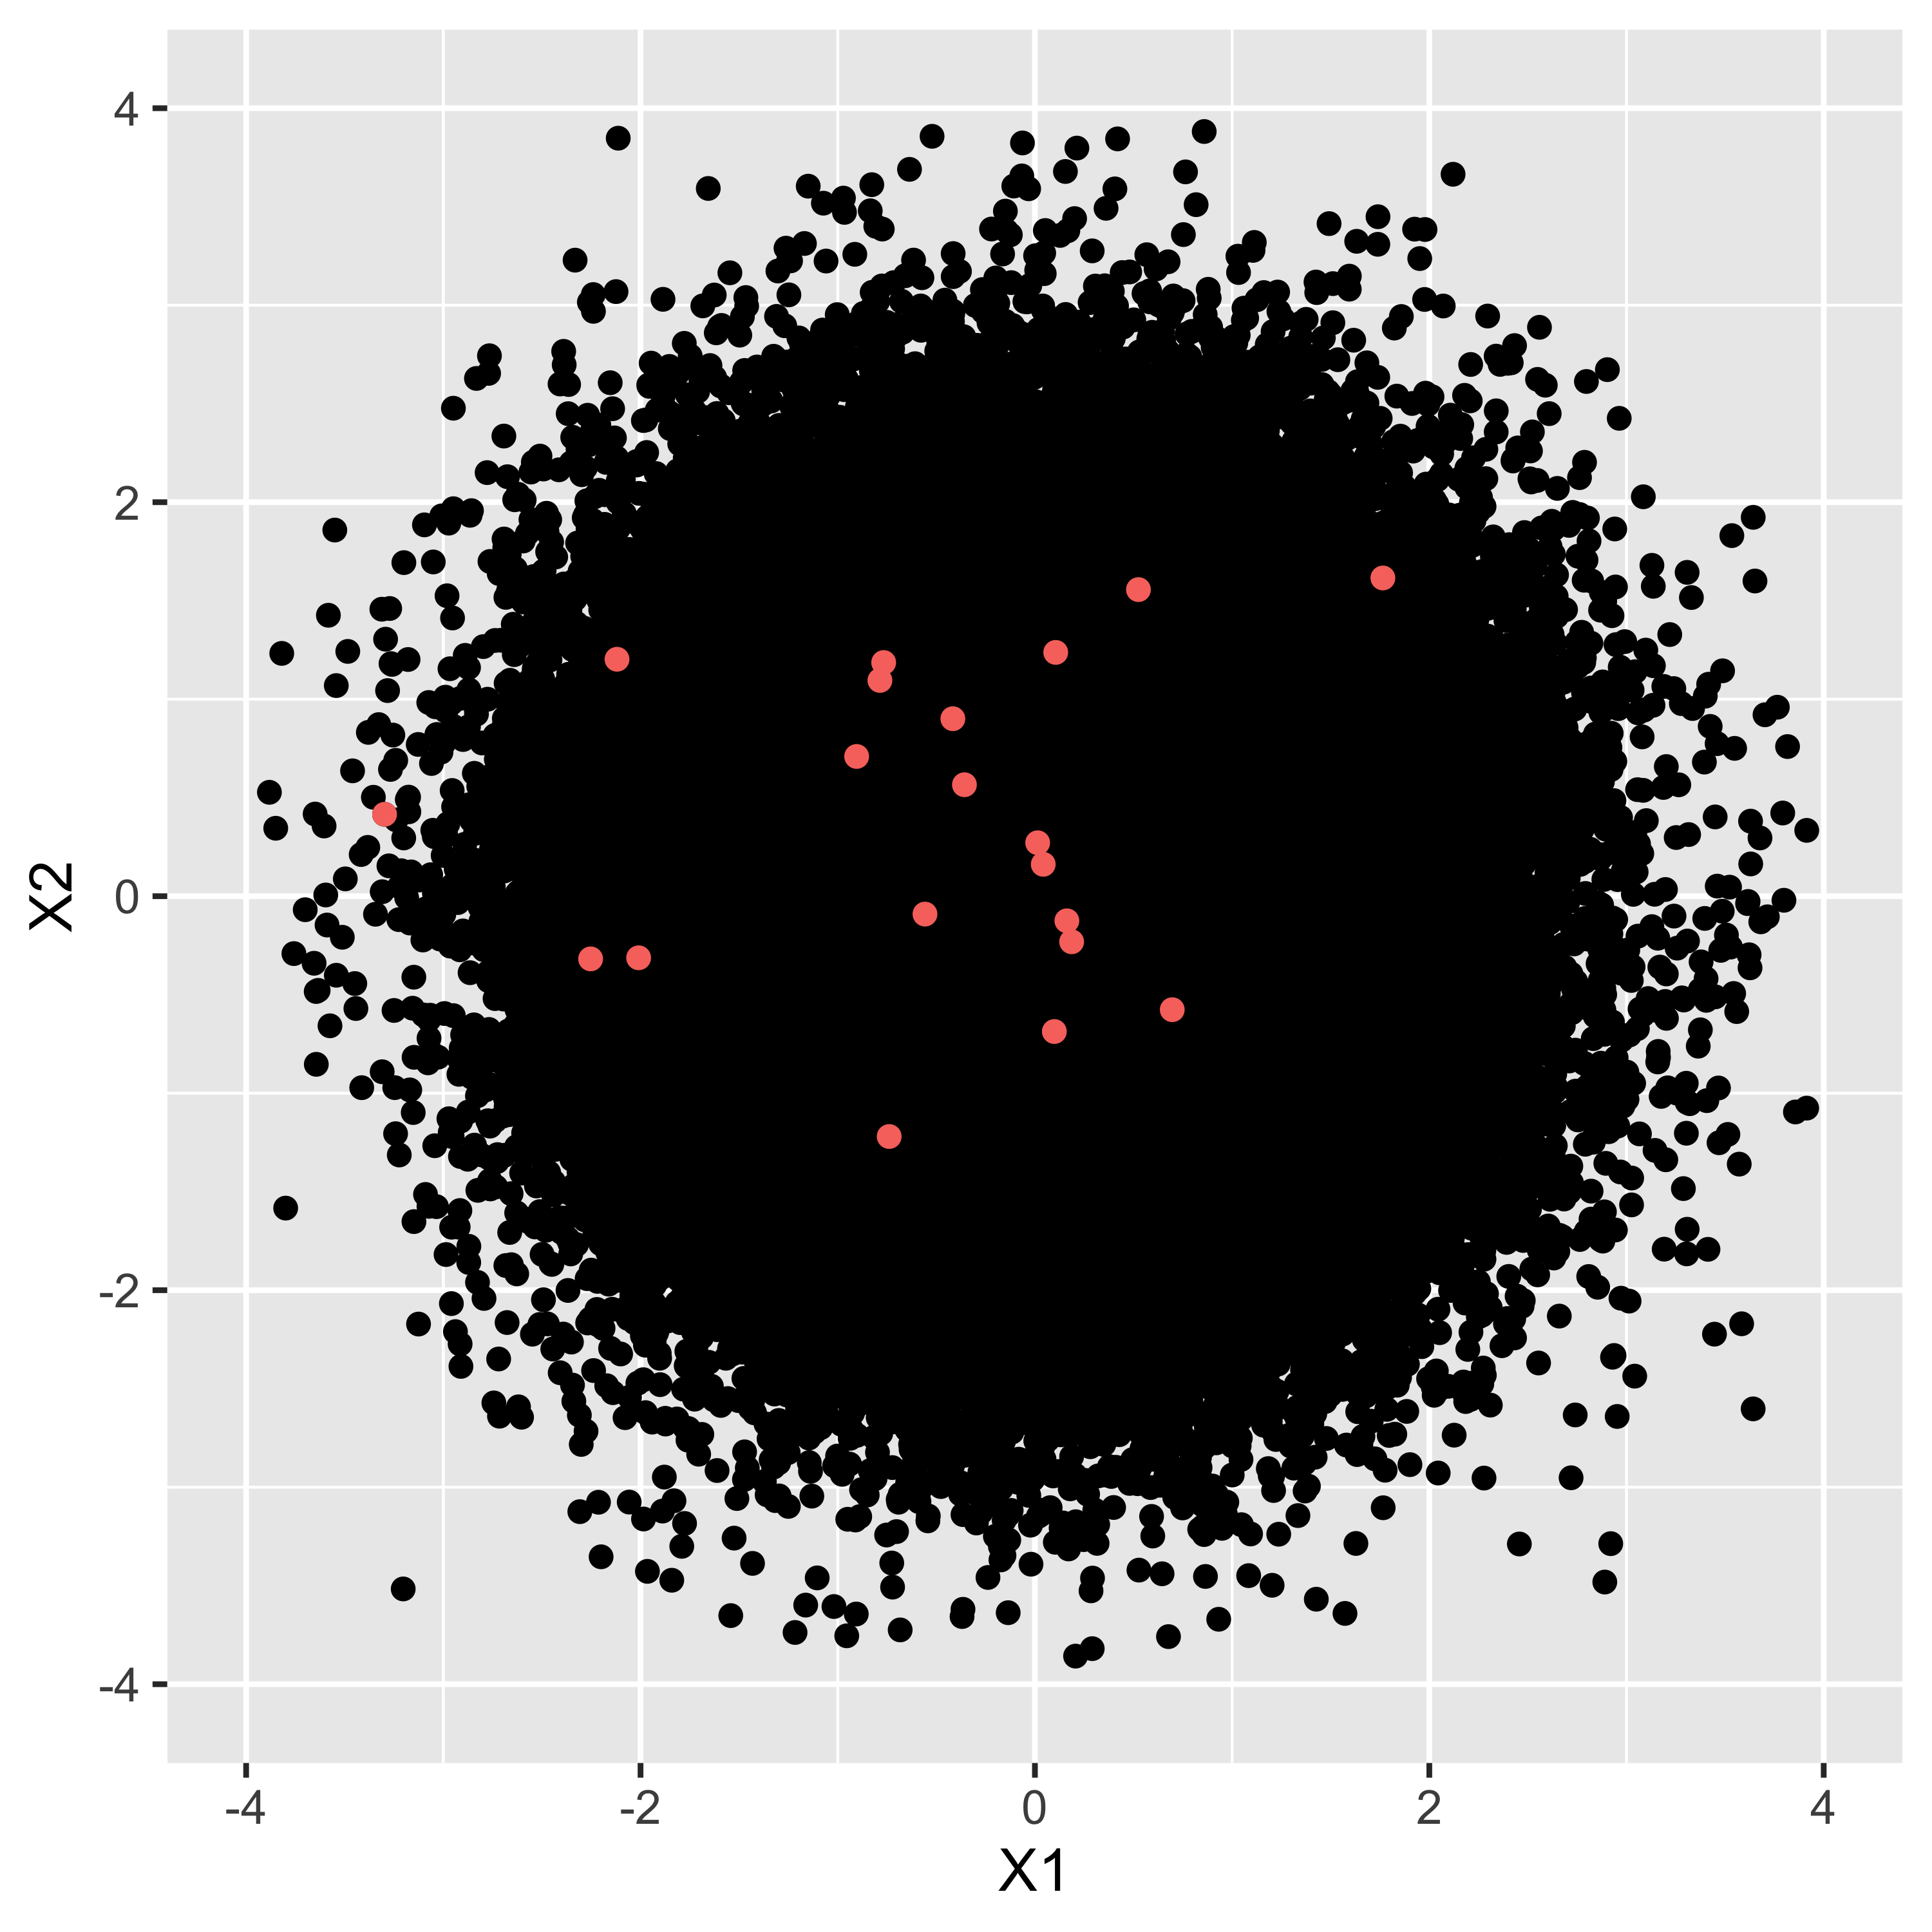
\includegraphics[keepaspectratio,width=0.8\linewidth]{figures/13_NHST/corr_sample20.png}
	\caption{母相関$\rho=0$の世界とそこから$n=20$のサンプルを取った例}
	\label{fig:13_01}
\end{figure}

図\ref{fig:13_01}に示したのは，母相関$\rho=0$の世界から乱数を10万点発生させ，そこからランダムに20個の点を取り出した例です。黒い点の塊はほぼ円で，二変数に相関がないというデータを具現化したものが示されています。小さな赤い点がそこから20個取り出した場合で，今回この20個の点による標本相関係数は$r=0.143$でした。理論的には$\rho=0$の世界からのサンプルなのですから，$r$も0であって欲しいかもしれませんが，一部の標本だけ取り出すとぴったり0になることはありません。同様のサンプルを何度も繰り返すと，標本相関係数は$r_2=0.32, r_3=-0.46,r_4=-0.26....$といろいろな数字を取ります。この分布が標本分布になるのです。

このように，いったん「母相関は$\rho=0$」，としてから標本を取り出したとして，その標本分布がどうなるかを考え，たまたま今回得られた標本相関係数(今回の例では0.5でしたが)が出てくる確率はどれぐらいか，を考えます。その確率が非常に小さければ，滅多にないことが目の前のデータで生じたわけですから，これは前提である「母相関は$\rho=0$」という仮定の方がおかしい，ということで帰無仮説を捨てるわけです。ここが背理法になっているわけですね。また，帰無仮説として「母相関はありまぁす！」という仮定を置くのも難しいところなのがわかっていただけるかと思います。相関が「ある」といって，どの程度あるのかは無数に考えられるのに対し，相関が「ない」の場合は一意に定まるからです。

\paragraph{検定統計量を定める}

ここで，標本相関係数の標本分布は，自由度$n-2$の$t$分布に従うことがわかっています\footnote{なんだそれ！と思った人もいるかもしれません。どうして平均値の推定に使った$t$がここでも出てくるのか，という問題は興味深く，この話をするには数理統計学の話題を持ってくる必要がありますが，流石にそれは寄り道しすぎなので，数理統計学に感謝して先に進みましょう。}。ただ，そのまま相関係数を使うのではなくて，標本相関係数を次の式で変換する必要があります。

\[ t = \frac{r\sqrt{n-2}}{\sqrt{1-r^2}} \]

\paragraph{判断基準の設定}
今回も慣例に倣って0.05(5\%)にしましょう。

\paragraph{検定統計量の算出}

今回の例では，

\[ t = \frac{0.5 \times \sqrt{18}}{\sqrt{1-0.25}} = 2.44949 \]

となりました。

\paragraph{では判定を}

今回得られた数字，$t=2.45$よりも大きい数字が自由度18のt分布から出てくる確率はどれぐらいでしょう？ これを計算すると\footnote{Rで\texttt{1-pt(2.45,df=18)}とします。}その確率は$p=0.01237173$です。またここでは，$\rho=0.0$の元で標本相関係数が$0.5$より大きくなる確率を考えているのですが，この偏った相関係数の出方は$|r|>0.5$についての話ですから，左右対称の分布であることから$p=0.0124\times2=0.0248$と考えるべきです。いずれにせよ，絶対値0.5以上の標本相関係数が得られる確率は5\%よりも小さい数字で，勝負の判定としては「滅多にないことが起こった」と言って良いわけですから，これは帰無仮説がおかしい。そもそも母相関が$\rho=0$であれば，たまたま標本から相関係数$r=0.5$が出てくるなんて，ありえへん，というわけです。そこで結論は，帰無仮説の棄却，対立仮説の採択となります。図\ref{fig:13_02}にt分布，臨界値，実現値の関係を図示しましたので，確認しておいてください。

\begin{figure}[ht]
	\centering
	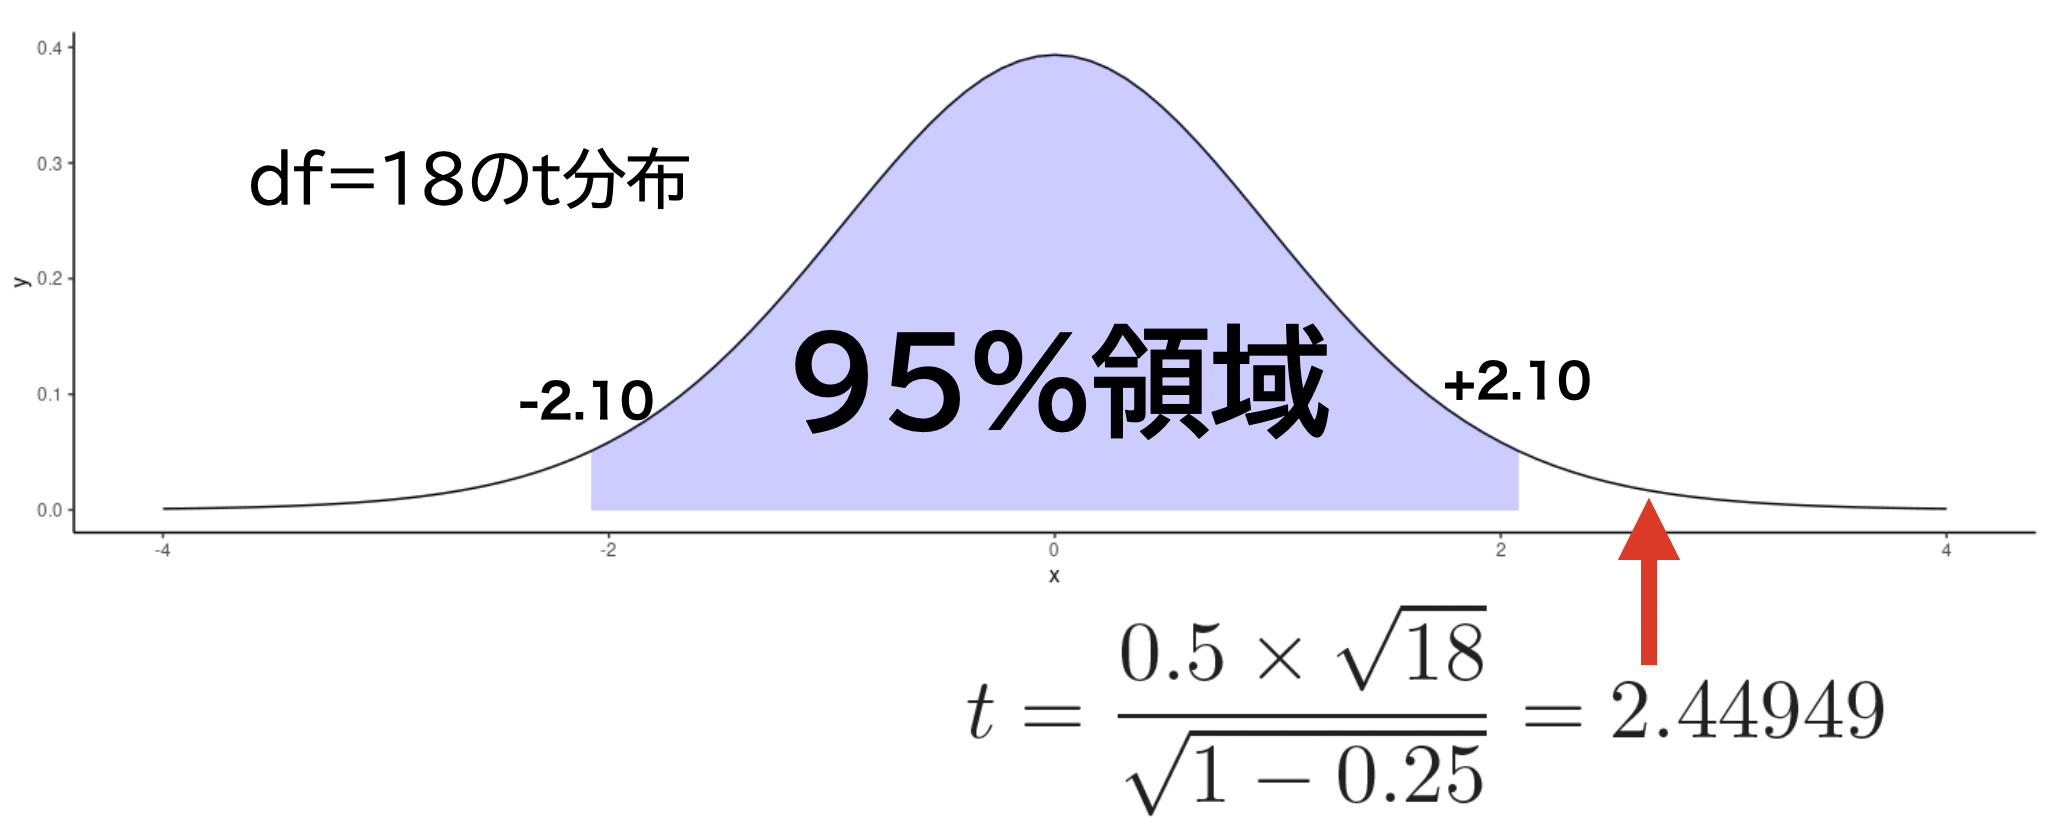
\includegraphics[keepaspectratio,width=0.8\linewidth]{figures/13_NHST/t_18_95.png}
	\caption{相関係数の検定結果をt分布で判断する}
	\label{fig:13_02}
\end{figure}

いかがだったでしょうか。帰無仮説検定は帰無仮説と対立仮説のモデル比較，仮想的な勝負であり，その判定の仕方を検定と呼ぶというのがお分かりいただけましたでしょうか。ちなみにここで有意かどうかの判断をしたことと，相関係数の大きさとは別の話です。サンプルサイズが非常に大きくなると，僅かな違いでも検出しやすくなり，例えば$r=0.01$でも有意になることがあります。つまり，帰無仮説検定は「差があるかないか」を判断するものであって，「どれぐらいの差があるか」を判断するものではないことに注意してください。

\section{$\chi^2$検定}

今度は$\chi^2$検定を考えてみましょう。セクション\ref{sec:chi_square},Pp.\pageref{sec:chi_square}で学んだように，$\chi^2$検定は度数のばらつきが期待値とどれぐらい違うかを検定する方法でした。ここでは，$\chi^2$検定を使って，度数分布の偏りがあるかどうかを判断する方法を考えてみましょう。

セクション\ref{sec:chi_square}でも紹介した，睡眠障害と年齢の関係のクロス集計表を例に取ります(表\ref{tab:age_sleep_re})。あらためて同じ表を掲載しますが，ここでは年齢層と睡眠障害の有無の関係を調べたのでした。年齢層は10代，20代，30代，40代以上の4つに分け，睡眠障害の有無は「あり」「なし」の2つに分けています。
% latex table generated in R 4.5.0 by xtable 1.8-4 package
% Sat May 17 13:32:22 2025
\begin{table}[ht]
\centering
\caption{年齢層と睡眠障害のクロス集計表} 
\begin{tabular}{rrrr}
  \hline
 & あり & なし & 合計 \\ 
  \hline
10代 & 8 & 30 & 38 \\ 
  20代 & 30 & 77 & 107 \\ 
  30代 & 27 & 60 & 87 \\ 
  40代以上 & 40 & 28 & 68 \\ 
  合計 & 105 & 195 & 300 \\ 
   \hline
\end{tabular}
\label{tab:age_sleep_re}
\end{table}

以前は，行や列の相対度数を見て考察したり，$\chi^2$値から\keyterm{クラメールのV}{くらめーるのぶい}{Cramér's V}を計算したりして，関係の強さを記述したのでした。$\chi^2$値が大きいとか，クラメールのVが大きいから関係があるんだ，というのはあくまでも記述的な話であり，大小の評価について客観的な基準が弱いともいえます。

そこで推測統計学的に，このようなクロス集計表の関係が偶然に生じたものではない，ということを検定してみましょう。

\paragraph{仮説の設定：クロス集計表の場合}
まずは仮説の設定です。クロス集計表の検定では，\keyterm{帰無仮説}{きむかせつ}{Null Hypothesis}は「行と列の度数分布は独立である」とします。つまり，両者は実は何の関係もなく，たまたまこのようなばらつきになったのだと考えるのです。
これに対して\keyterm{対立仮説}{たいりつかせつ}{Alternative Hypothesis}は「行と列の度数分布は独立ではない」，つまり何らかの関係がある，ということになります。

\paragraph{検定統計量を定める}

検定統計量はすでにサブタイトルにもあるように，$\chi^2$値を使います。

\paragraph{判断基準の設定}
今回も慣例に倣って0.05(5\%)にしましょう。

\paragraph{検定統計量の算出}

今回は$9.9627$になりました。計算の仕方はセクション\ref{sec:chi_square}で学んだ通りですが，実際はRが検定結果とともに算出してくれますので，それほど気にしなくて構いません。

\paragraph{では判定を}

ここで，$\chi^2$値がどれぐらいの確率で出てくるのかを計算します。自由度は$(行数-1)(列数-1)$として計算するので，今回は$3$になります。Rには次のように入力するといいでしょう。


\begin{lstlisting}[language=R,label={code:6_05},caption={クロス集計表の検定結果をRで計算する}]
cross <- matrix(c(8,30,30,77,27,60,40,28), ncol = 2, byrow = T) 
print(cross)
chisq.test(cross)
\end{lstlisting}

\paragraph{コード解説}
\begin{description}
    \item[1行目] \verb|matrix|関数で度数データを行列として作成します。\verb|c()|で数値を並べ，\verb|ncol=2|で2列，\verb|byrow=T|で行優先で入力します。今回はロウデータからクロス集計表を作成するので，このような形で作りましたが、実際は\verb|tables|関数などでデータから作ることが多いでしょう。
    \item[2行目] \verb|print|関数で作成した行列の内容を確認・表示します。
    \item[3行目] \verb|chisq.test|関数でカイ二乗検定を実行し，統計量と有意確率を算出します。
\end{description}

出力結果を見てみます(出力\ref{RS:chi-square_test})。
$\chi^2$値は$23.095$，自由度は$3$，そして$p$値は$3.858 \times 10^{-5}$となりました。これは非常に小さい数字で，5\%の有意水準を大きく下回っています。つまり，帰無仮説を棄却し，対立仮説を採択することになります。
つまり，年齢層と睡眠障害の有無には何らかの関係がある，と判断することになります。

\begin{Rscreen}{出力例}{chi-square_test}
\begin{verbatim}
> cross <- matrix(c(8,30,30,77,27,60,40,28), ncol = 2, byrow = T)
> cross
     [,1] [,2]
[1,]    8   30
[2,]   30   77
[3,]   27   60
[4,]   40   28
> chisq.test(cross)

        Pearson's Chi-squared test

data:  cross
X-squared = 23.095, df = 3, p-value = 3.858e-05
\end{verbatim}
\end{Rscreen}



\section{1つの平均値の検定}

次に，心理学で最もよく使われる検定の一つである，平均値の検定についてみていきます。実践的には複数の群の平均値を比較することが多いのですが，まずは1つの平均値の検定から始めていきましょう。

まずは平均値の推定の時と同じく，母集団のSDがわかっている場合に標準正規分布を使っての検定を，次に母集団のSDがわからない時の，t分布を使っての検定を見ていくことにします。
\subsection{母SDがわかっている場合}
% ではまず，1つの平均値の推定を使って，検定をしてみましょう。「推定を使って検定」というのは変な表現に聞こえるかもしれませんが，推定は「母数はこれぐらいではないか」という予測の話であり，検定は「母数がそのようであれば，このように結論づける」という意思決定の話なのです\footnote{意思決定なんかしなくていいじゃない，と思うかもしれません。確かに科学的探究であれば，母数がどの程度であるかというのを知ることで十分なのです。しかし，帰無仮説検定は農学で生まれ，医学領域にも広まっている技術です。これ以上実験を続けて良いかどうか，この治療薬を投与し続けて良いかどうか，といった実際的な問題がそこにはあり，効果があるとしたらこれぐらい，ない可能性もなくはない...という態度を続けていると前に進まないので，何らかの基準が必要だという事情もあります。心理学においても，より実際的な場面では意思決定が必要になることもありましょう。}。

さて，話を進めるために，具体的な例をあげてみましょう。ある学校で，学力テストしたとします。その学校で無作為に49人分の記録を取り出したところ，平均が52点でした。このテスト，全国平均は50点で，SDが9の正規分布であることがわかっていたとします。これとそのまま比べると，その学校の成績が良い，ということになりますが，たった2点差でそのように結論づけて良いかどうか，というのがここでの問題です。

帰無仮説検定のステップを思い出しましょう。まずは仮説を設定します。
ここでやりたいことは，「この学校の成績が良いかどうかの判断」です。言い換えると，全国平均の分布が母集団でそれの平均やSDがわかっているのですから，この標本の平均は母平均と同じなのか，異なっているのかが知りたいのです。標本ですからたまたま高い点数が出ること(そしてその逆)もありますが，この標本平均から推測される母平均と，このテストの理論的な平均値(全国平均)の違いが\textbf{統計的に有意な差なのかどうか}が知りたいわけです。数式で表現すると，標本平均は$\bar{X}$で，$\bar{X} \sim N(\mu, \frac{\sigma}{\sqrt{n}})$ですから，この時の$\mu=50$が帰無仮説，$\mu \neq 50$が対立仮説ということになります。

次に検定統計量ですが，平均値の推定，しかも理論的に平均50，SD9の正規分布との照合ですから，推定したい対象の特徴がもうわかっている特殊なケースです。これは変換すれば標準正規分布に従うのですから，標準化されたZ得点が検定統計量になります。

第3のステップは基準になる確率を設定する，でした。勝敗を決めるルールの決定ですね。これはとくに意味もなく，慣例に従って0.05(5\%)としておきましょう。

これで準備が終わりました。実際の検定統計量の計算です。平均$\mu$，分散$\sigma^2$の正規分布する母集団からの標本の場合，標本平均の標本分布も正規分布に従い，
\[ \bar{X} \sim N(\mu,\frac{\sigma}{\sqrt{n}}) \]
になります。今回の場合は，
\[ 52 \sim N(50,9/\sqrt{49}) \]
だと考えられます。標準化することで標準正規分布を使うことができますから，
\[ (52-50)/(9/7) \sim N(0,1) \]
として，$ (52-50)/(9/7) =2/1.285714=1.555... $を得ます。この1.556(下三桁までで四捨五入しました)という数字はどのあたりに位置するのでしょう？

そこで確率の計算をしてみましょう。これが次のステップの，実際のデータから検定統計量の実現値を計算する，というやつです。標準正規分布において，1.556より大きな数字が得られる確率は\footnote{これまた確率の，とくに連続変数のややこしいところで，1.556という数字が出てくる確率はゼロです。ユークリッド幾何学でいうところの，点は位置があって大きさがないというのと同じで，点の確率は大きさがないのです。確率は面積ですから，1.556\underline{より大きな数字}が得られる確率，というのが本当は正しい表現です。}，$p=0.05985405$でした\footnote{これはRで次のように計算しています：\texttt{1-pnorm(1.556,mean=0,sd=1)}}。5.9\%なのですね。

最後に判定です。5\%が判定ラインだったわけですが，今回得られた「確率変数の実現値」は5\%より大きな確率です。つまり大きい＝出現する可能性が大きい，よくある話だったわけです。そんなにレアな数字じゃない。つまり，たまたま今回の標本が，平均から2点大きくなるようなことは十分あり得る話だということです。この学校の生徒は優秀だー！と言いたいところなんですが，偶然それぐらいの差がでることがあるのであれば，そこまで胸を張っていうことができません。ということで，軍配としては帰無仮説の勝ち，つまり，「その学校の成績が特段良いわけではない」「統計的には差がない」ということになります。

図で確認しておきましょう。図\ref{fig:13_03}には標準正規分布と今回の判定に係る数字を記載しました。今回計算した統計量は，標準正規分布にしたがいます。標準正規分布で5\% という基準を考えると，$\pm1.96$を超えた領域になります。今回のデータがこの領域に入るほどのものであれば，帰無仮説は棄却することになりますが，今回はその領域に入らない，つまり「このサンプルからこの平均値が出てくることも，あるよ」ということで棄却できないのでした。帰無仮説を棄却する領域のことを一般に\keytermL{棄却域}{ききゃくいき}といい，この数字を越えれば棄却域に入るというギリギリの数字のことを\keytermL{臨界値}{りんかいち}といいます。今回の臨界値は$\pm1.96$で，両端が棄却域，今回の1.55という実現値は棄却域に入らなかったので帰無仮説の勝ち，ということです。
\begin{figure}[ht]
	\centering
	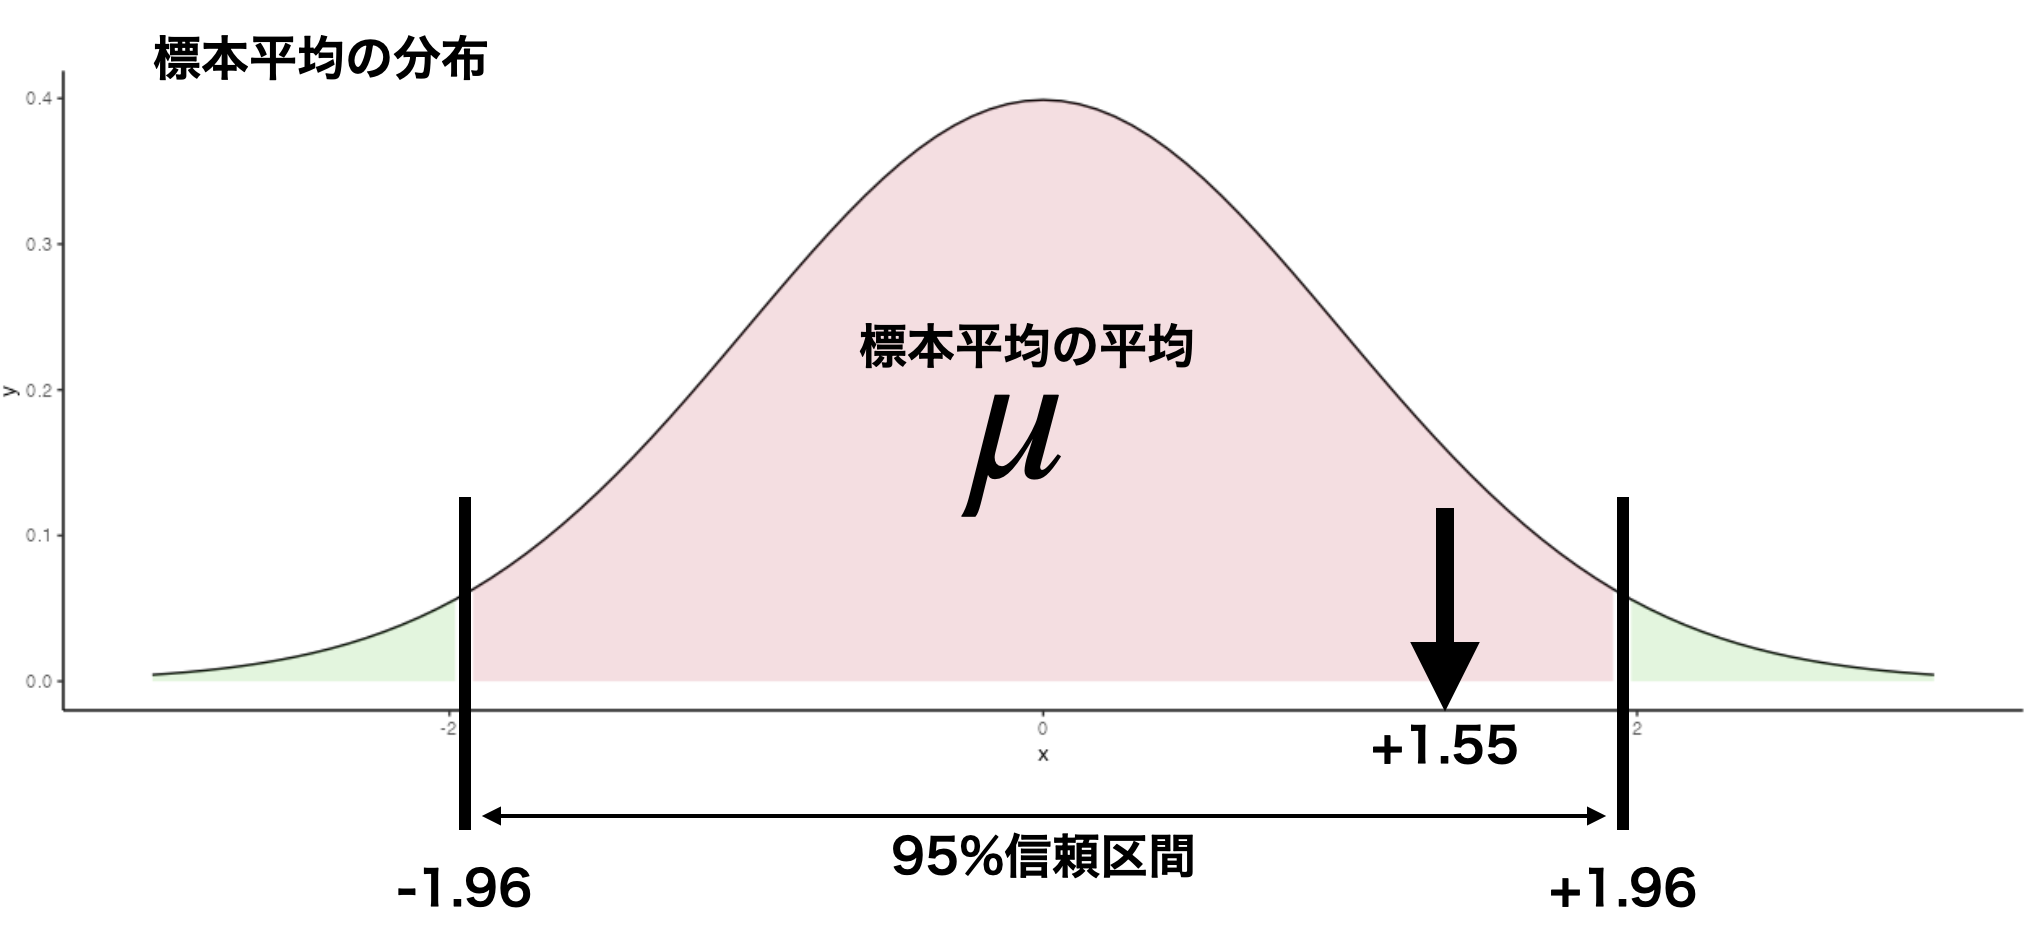
\includegraphics[keepaspectratio,width=0.8\linewidth]{figures/13_NHST/normal_95.png}
	\caption{棄却域と臨界値}
	\label{fig:13_03}
\end{figure}


\subsection{母SDがわかっていない場合}
先ほどの例は，母SDがわかっているという話でした。まあ母数がわかっていれば苦労はないわけで，それが分からないから推測するのですよね。

ということで，母SDの代わりに標本SD(\keytermL{不偏分散}{ふへんぶんさん}の正の平方根)を使って推定することとします。そのさいは(標準)正規分布が使えないので，サンプルサイズに応じた$t$分布を使うのでした。同じデータ例でやってみましょう。今度は標本の標準偏差が必要ですので，これが$\hat{\sigma}=10$だったとします。

帰無仮説・対立仮説はさきほどと同じく，$\mu=50$か$\mu \neq 50$です。ただし推測に使う統計量が$t$になるわけです。
判断基準も同じく慣例にならって，なんとなく5\%にしておきましょう。
検定統計量$t$は$t = \frac{\bar{X}-\mu}{\hat{\sigma}/\sqrt{n}}$で求めることができますから，
\[ t = (52-50)/(10/7) = 1.4 \]
となります。これが自由度$n-1=48$の$t$分布に従うので，自由度48の$t$分布において1.4以上の数字が出る確率を求めますと，$p=0.08397194$となりました\footnote{これはRで次のように計算しています：\texttt{1-pt(1.4,df=48)}}。8.3\%なのですね。

これで判定です。5\%の判定ラインより大きな確率が出ましたので，これは滅多にないことではない。なくはないのだから，よくある話。珍しいことじゃない。つまり，母平均から外れて大きい数字，とまでは言えないねということになります。
今回の判定に関するイメージを図\ref{fig:13_04}に示しました。今回は自由度48のt分布を描き，検定統計量の実現値を示しています。実現値が棄却域に入るか入らないか，という判断をしてもいいですし，今回のように直接確率を算出して5\%になるかどうかの判定をしてもらっても結構です\footnote{直接確率を計算する方が楽なのに，と思う方もいるかもしれません。これは歴史的な経緯があって，今でこそRなどを使って簡単に確率点が計算できますが，そういう機械がなかった頃は数字の表を見て判断していたのです。第\ref{ch10_probability}講義のセクション\ref{10::number_table},Pp.\pageref{10::number_table}で数表のことをご紹介しましたが，あれを見て臨界値の大小で棄却域に入ったかどうかを判断する，というのが一般だった時の名残だと思ってください。}。
\begin{figure}[ht]
	\centering
	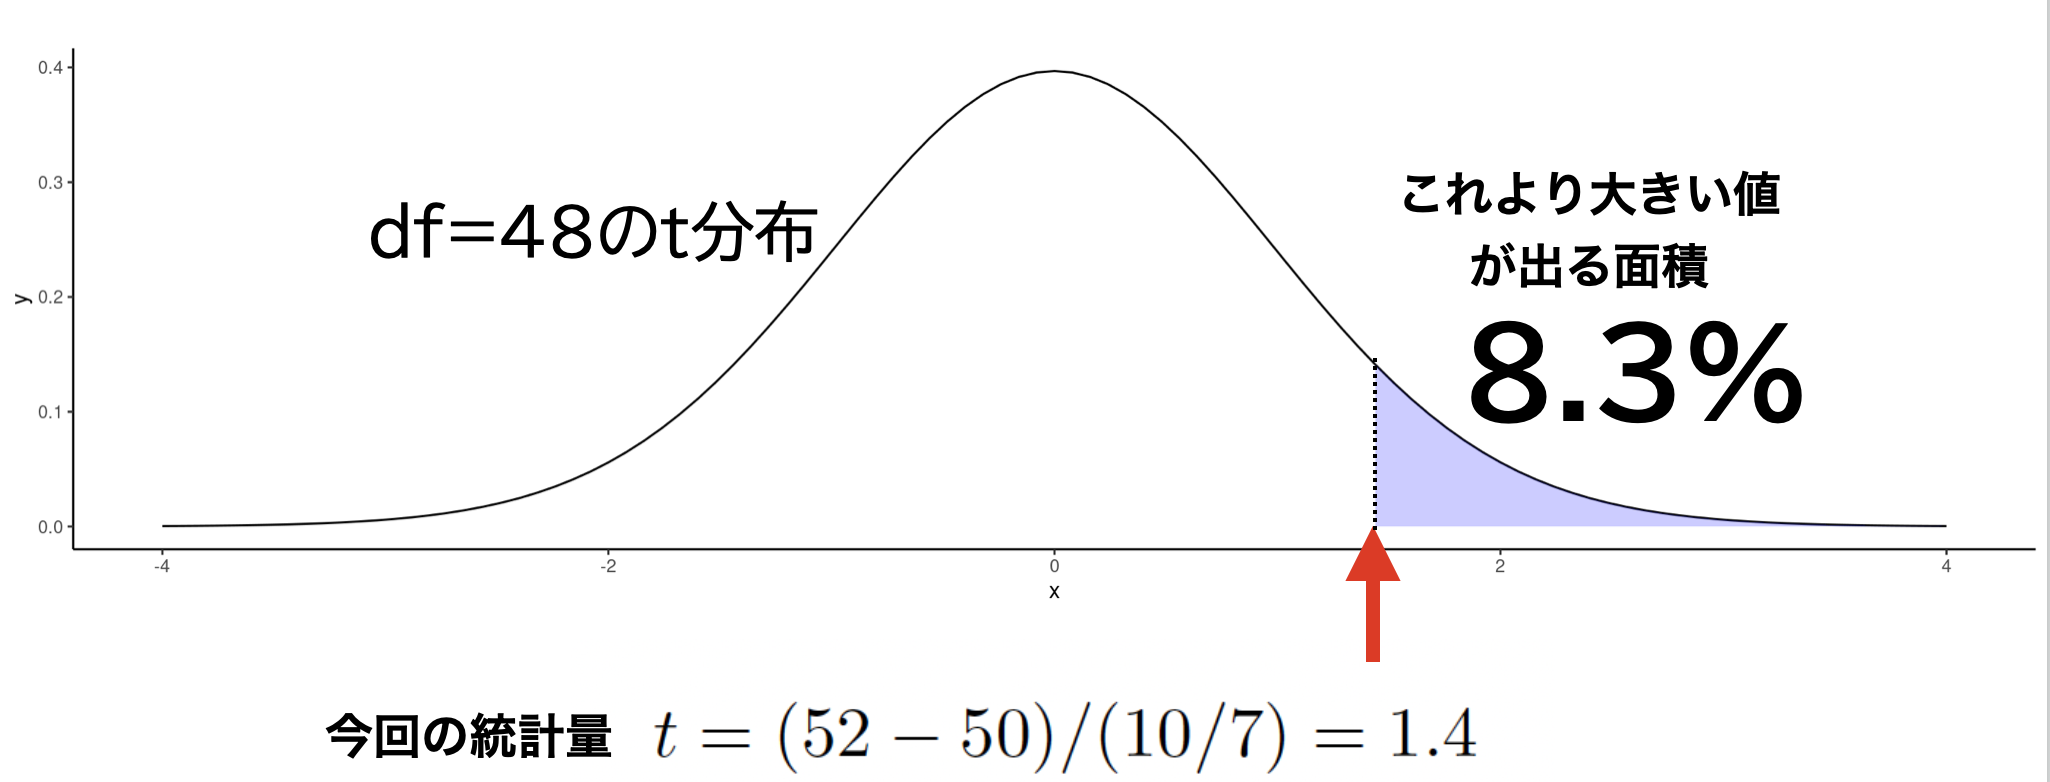
\includegraphics[keepaspectratio,width=0.8\linewidth]{figures/13_NHST/t8_3.png}
	\caption{t分布をつかったときの棄却域と臨界値}
	\label{fig:13_04}
\end{figure}


いかがでしたでしょうか。今回のデータでは(母SDがわかっていても，わかっていなくても)帰無仮説を棄却することはできませんでした。何だか持って回った言い方をしているように感じられるかもしれませんし，いまいちイメージが掴みにくいかもしれません。そこで，今度はまた別のケース，相関係数の例で考えてみたいと思います。徐々に手続きと結論の出し方に慣れていくと思います。


\section{結果の報告の仕方}
帰無仮説検定は帰無仮説と対立仮説のモデル対決なので，結果は軍配をはっきり示す必要があります。帰無仮説が勝ったのか，対立仮説が勝ったのかを明記するのです。ちなみに仮説が勝った，というのを\keyterm{採択}{さいたく}{accept}，負けたというのを\keyterm{棄却}{ききゃく}{reject}と言うのでした。ですから「帰無仮説を棄却して対立仮説を採択」，あるいは「帰無仮説が棄却できずに採択，対立仮説を棄却」のどちらかになります。

また，結果の判定ですから，判定に使った数字＝検定統計量も報告する必要があります。たとえば相関係数の検定の例では，$t$統計量が使われましたので，これを報告します。また，$t$統計量は$t$分布に従い，これはサンプルサイズに依存する自由度によって調整されるものですから，自由度も報告する必要があります。前回の例では，相関係数$r=0.50$がサンプルサイズ20のデータから得られ，統計的に有意であると結論づけられたのでした。この結果は，次のように報告しましょう。
\begin{quote}
	標本から得られた標本相関係数$r=0.50$について仮説検定を行ったところ，$t(18)=2.450,p=0.0248$で統計的に有意であった。
\end{quote}
書き方のポイントとしては，統計量を書くこと，そしてその時の統計量はイタリック(斜体)であること\footnote{字体を整えるのは，心理学だけでなく論文の書き方として一般的です。統計量や本のタイトルなどはイタリックであることが決まっています。誰が決めているかって? America Psychological AssociationのPublication Manualにそう定められていますし，日本の心理学会も基本的にこれに準じた出版作法を定めているのです。}，その統計量の実現値が得られる確率($p$値)を記載すること，です。

$p$値は上の例のように確率そのものを描くのが基本ですが，昔は判定基準を使って$p<0.05$とか$p<0.01$と書いていました。これは手計算で検定をしていた頃の名残で，統計環境Rなどがなかったものですから確率計算が直接できませんでした。ではどうしていたか，というと代表的な確率分布の数字が載っている数表\footnote{昔は確率分布の数字の一覧が載っている本がありました。確率のテキストには付録として，数表の一部が載っているものもあります。}を使ってチェックするしかなかったので，細かい数字まで計算できなかったのです\footnote{たとえばt分布は自由度によって変わりますが，自由度$1,2,3\cdots$と1つずつ書いてあったのでは，付録のページ数がいくつあっても足りません。そこで$1,2,3...10,15,30,50$のように，後半の方は「だいたいこれぐらい」という大雑把な幅でしか載っていませんでした。こんな時，じゃあ自由度18ならどうしたらいいんだ，と思うかもしれませんが，その時は手元のデータに最も近く，より厳しい自由度15のところを見て代替する，というやりかたでした。ですから具体的な$p$値は書けなかったのです。}。今ではそういう問題がないので，そのまま$p$値を書きましょう。

\end{document}
